\documentclass{beamer}

% \usepackage{beamerthemesplit} // Activate for custom appearance
\usepackage{hyperref}

\title{Working with 3rd Party APIS}
\author{Katie Ford}
\date{\today}

\begin{document}


\frame{\titlepage}

\section[Outline]{}
\frame{\tableofcontents}

\section{APIs - What are they?}
\frame{
	\frametitle{What is an API?}
	\pause
	\begin{itemize}
	\item "Application Programming Interface"
	\item 3rd-party Web APIs
	\item REST, SOAP
	\end{itemize}
}

\frame{
	\frametitle{How do they get information?}
	\begin{itemize}
		\item HTTP(S) Requests
	\end{itemize}
}

\frame{
	\frametitle{How do we get information back?}
	\begin{itemize}
		\item text
		\item Serialization: json, xml, yaml, custom
	\end{itemize}
}

\section{How to work with it}
\frame{
	\frametitle{SDKs, packages, and libraries. Oh my!}
	\begin{itemize}
		\item Advantages: easy to use, pre-built
		\item Disadvantages: limited languages, dependencies
	\end{itemize}
}
\frame{
	\frametitle{OAuth}
	\begin{center}
		\hyperref[OAuth introduction]{https://oauth.net/about/introduction/}\\
		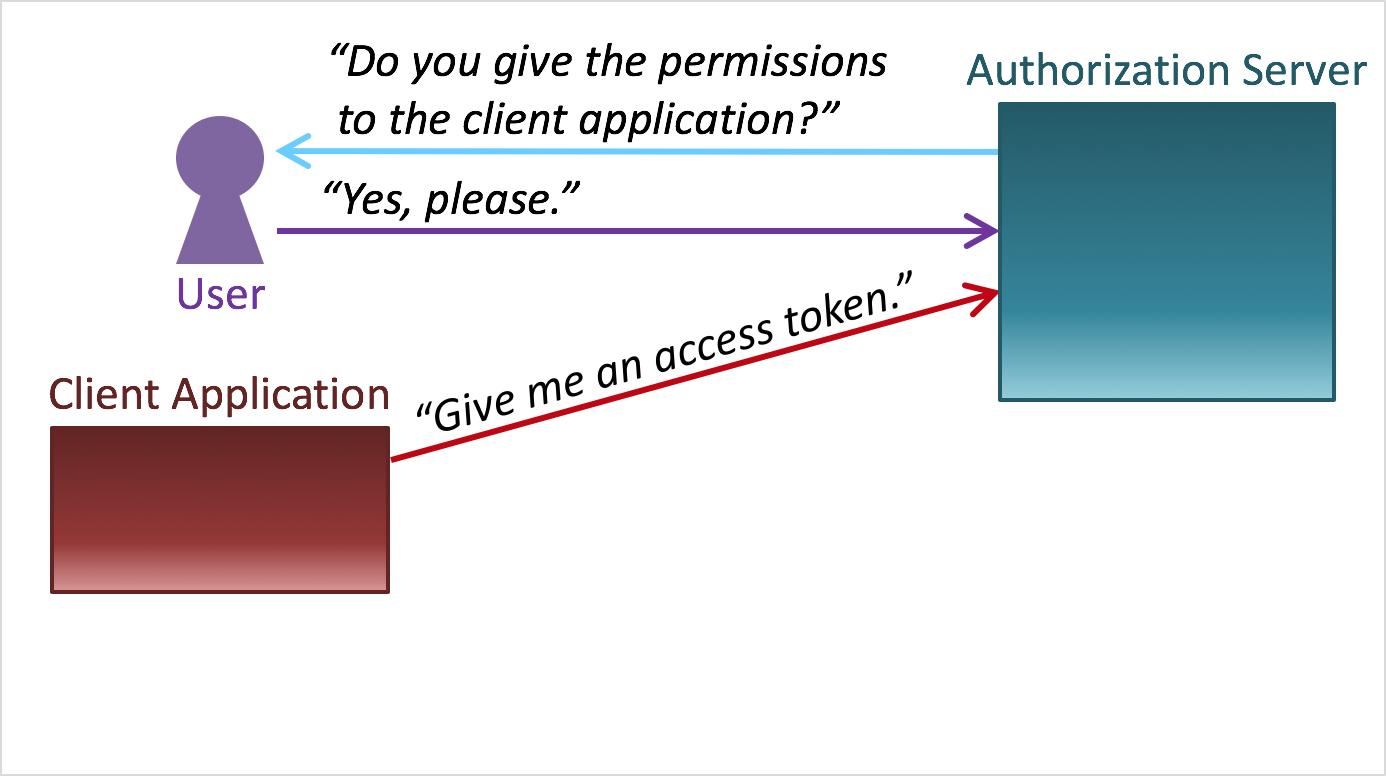
\includegraphics[width=4cm]{oauth_explained.png}
	\end{center}
}

\section{Intermediate Gap}
\frame{
	\frametitle{Wait, what?}
	\begin{center}
		
\includegraphics[width=4cm]{confusedladymathmeme.png}
	\end{center}
	\begin{itemize}
		\item Finding something I cared about
		\item Abstractions on abstractions
	\end{itemize}
}
\frame{
	\frametitle{Code!}
	
}
\frame{
	\frametitle{Auth files}
	\begin{itemize}
		\item /etc/auth directory
		\item .gitignore
	\end{itemize}
}

\section{More!}
\frame{
	\frametitle{Me}
	\begin{itemize}
		\item https://github.com/ClassicKatie/wwcode-api
		\item @Classic\_Katie
		\item katie@womenwhocode.com
		\item katie@katieford.io
		\item Slack
	\end{itemize}
}

\end{document}
